\documentclass[tikz]{standalone}
\usepackage{pgfplots}
\pgfplotsset{compat=1.15}
\usepackage{mathrsfs}
\usetikzlibrary{arrows,calc}
\usepackage{tkz-euclide}
\pagestyle{empty}

\definecolor{AngleClr}{rgb}{0,0.39215686274509803,0}
\definecolor{ShapeClr}{rgb}{0.6,0.2,0}

\begin{document}

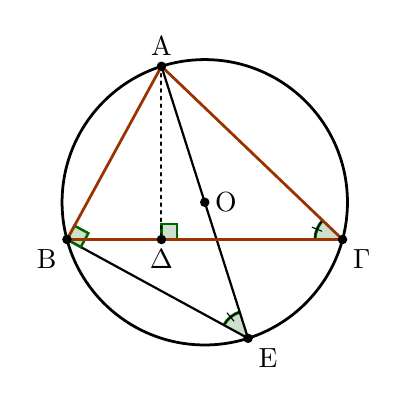
\begin{tikzpicture}[scale=1]
\tkzSetUpLine[line width=1pt,color=black]
\tkzSetUpPoint[fill=black]

\tkzDefPoints{0/0/B,3.5/0/C,1.2/2.2/A}

\tkzDefCircle[circum](A,B,C) \tkzGetPoint{O}
\tkzDrawCircle[line width=1.0pt, color=black](O,A)

\tkzInterLC(A,O)(O,A) \tkzGetPoints{E}{X}
\tkzDefPointBy[projection=onto B--C](A)\tkzGetPoint{D}

\tkzFillPolygon[fill=white](A,B,C)

\tkzFillAngles[fill=AngleClr,size=.35,fill opacity=0.2](A,E,B A,C,B)
\tkzMarkAngles[line width=1.1pt,size=.35,color=AngleClr](A,E,B A,C,B)
\tkzMarkAngles[size=.35,mark=|,mksize=2](A,E,B A,C,B)

\tkzDrawSegments[line width=0.8pt,color=black](A,E B,E)


\tkzMarkRightAngles[line width=0.9pt, size=.2,color=AngleClr,fill=AngleClr,fill opacity=0.2](A,B,E A,D,C)

\tkzDrawSegment[line width=0.75pt,color=black,dashed,dash pattern=on 1pt off 1.75pt](A,D)

\tkzDrawPolygon[color=ShapeClr](A,B,C)
\tkzDrawPoints[size=3](A,B,C,O,D,E)
\tkzLabelPoint[below right](C){$\rm \Gamma$}
\tkzLabelPoint[above](A){$\rm A$}
\tkzLabelPoint[below left](B){$\rm B$}
\tkzLabelPoint[right](O){$\rm O$}
\tkzLabelPoint[below right](E){$\rm E$}
\tkzLabelPoint[below](D){$\rm \Delta$}


\end{tikzpicture}
\end{document}
